\chapter{Návod k použití}
\label{chap:howto}

\section{Instalace}

Nejprve je nutné nainstalovat runtime pro Python a Javascript.

\begin{itemize}
	\item Node.js 18
	\item Python 3.10
\end{itemize}

Pak je potřeba nainstalovat Mozaik. Přesný postup je uveden v jeho dokumentaci\cite{MozaikReadme}.

Dále doinstalujeme pip a npm balíčky.

\begin{lstlisting}[language=bash]
	pip install -r requirements.txt
	npm i -g @angular/cli
	cd frontend
	npm i
\end{lstlisting}

Ve stejné složce frontend zkompilujeme.

\begin{lstlisting}[language=bash]
	npm run build
\end{lstlisting}

\section{Spuštění}

Pro snadné spouštění je v kořenovém adresáři připraven skript \lstinline|run.sh|. Má několik volitelných parametrů.

\begin{lstlisting}[language=]
Start up flask server for mozaik visualization
Usage: ./run.sh [options]

Options:
		--expose
				listen on all network interfaces (default false)
		-h, --help
				display this message
		--port
				port to listen on (default 5000)
		--prod
				use production parameters (default false)
		--restart
				restart on crash (default false)
		--root
				root folder for looking up datastores,
				can be specified multiple times (default .)
\end{lstlisting}

\section{Testy}

Testy lze zvlášť spouštět pro Python a pro Angular.

\begin{lstlisting}[language=bash]
	pytest
	cd frontend
	npm run test
\end{lstlisting}

Angularové testy ze své podstaty musí běžet v prohlížeči. Adresa k otevření je vypsaná ve výstupu testovacího příkazu.

\section{Dev server}

Při vývoji Angularové části je doporučeno používat Angular dev server. Spustí se následujícím příkazem.

\begin{lstlisting}[language=bash]
	cd frontend
	npm run start
\end{lstlisting}

Tento server generuje sourcemaps pro snazší debugování, má zapnutou podporu pro store devtools, rekompiluje se při změnách kódu a automaticky přenačte otevřenou stránku. I nadále je ovšem potřeba mít spuštěný Flask server pro poskytnutí API.

\section{Základní práce s programem}

Protože program má grafické rozhraní, bylo by poněkud nešikovné bavit se o jeho používání jenom v textu. Následující část tedy bude sekvence obrázků, které nás provedou od načtení stránky po jednotlivé vizualizace. Aby byly dobře vidět, jsou některé screenshoty pořízeny na malé obrazovce. Při standardním běhu je na všechno více místa.

\begin{figure}
	\centering
	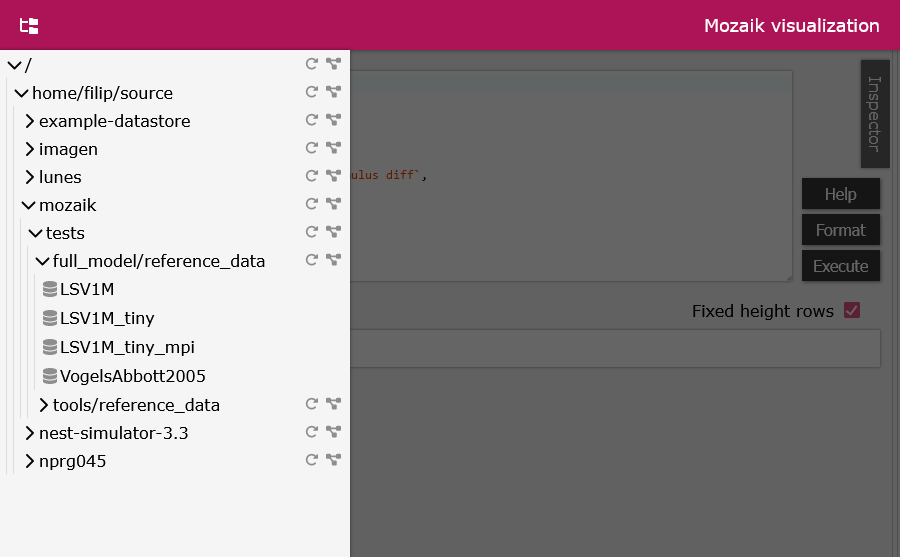
\includegraphics[width=1\linewidth]{img/screenshot_filesystem.png}
	\caption{Po načtení programu se zobrazí prohlížeč adresáře. Před další prací je nutno najít a vybrat datastore. Jednotlivé složky je možné procházet. Každá složka má navíc dvě tlačítka vpravo --- jedno z nich přenačte obsah složky a druhé její obsah načte rekurzivně a vyfiltruje složky bez datastore. Rekurzivně načtená byla složka \lstinline|mozaik|, proto jsou názvy některých složek v ní ve skutečnosti delší cesty.}
	\label{fig:filesystem}
\end{figure}

\begin{figure}
	\centering
	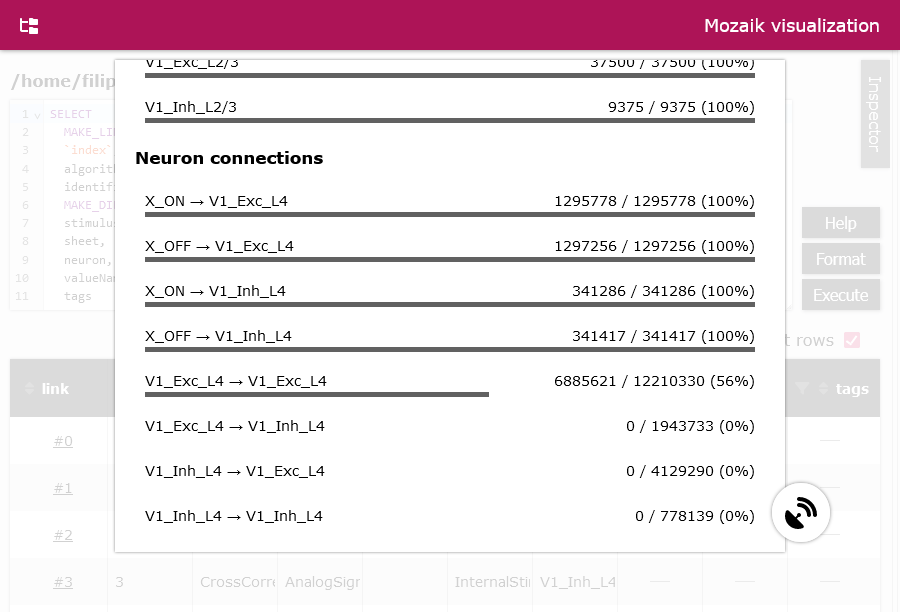
\includegraphics[width=1\linewidth]{img/screenshot_loading_model.png}
	\caption{Jakmile je datastore zvolen, načte se model. Při jeho načítání je vidět, kolik dat už se stáhlo. Vpravo dole je tlačítko, které zobrazí probíhající síťové dotazy --- to se zobrazí při jakékoli komunikaci po síti.}
	\label{fig:loading-model}
\end{figure}

\begin{figure}
	\centering
	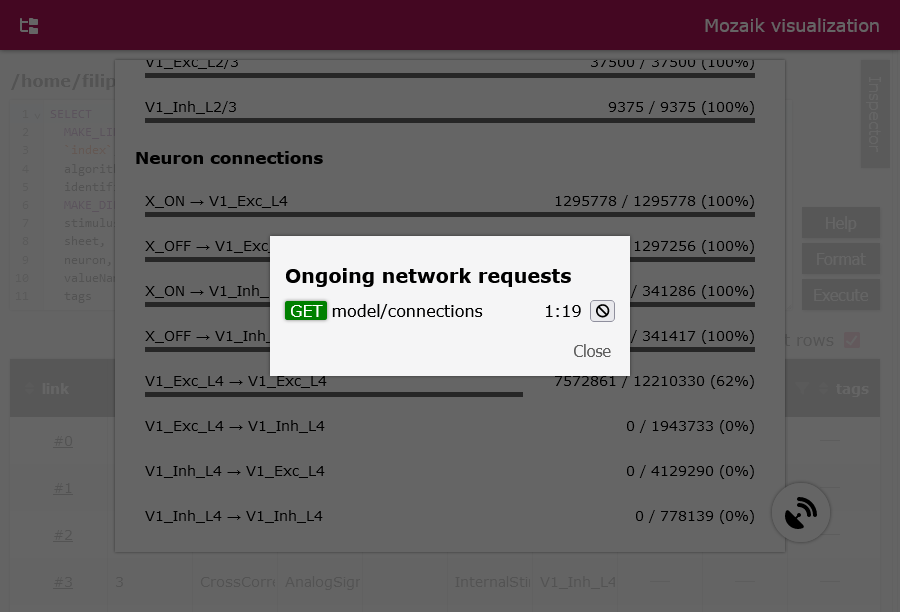
\includegraphics[width=1\linewidth]{img/screenshot_network.png}
	\caption{V tomto dialogu jsou vypsané jednotlivé probíhající dotazy. Dotaz může selhat a být spuštěn znovu, v takovém případě se zde ukazuje i o kolikátý pokus jde. Po kliknutí na tlačítko lze dotaz zrušit. To je vhodné v případě, že nejde o první pokus a dotaz zahrnuje hodně dat. Může to totiž znamenat, že byl server přetížen, došla mu paměť a byl mezitím restartován. Takový dotaz by akorát způsobil další restart serveru.}
	\label{fig:network}
\end{figure}

\begin{figure}
	\centering
	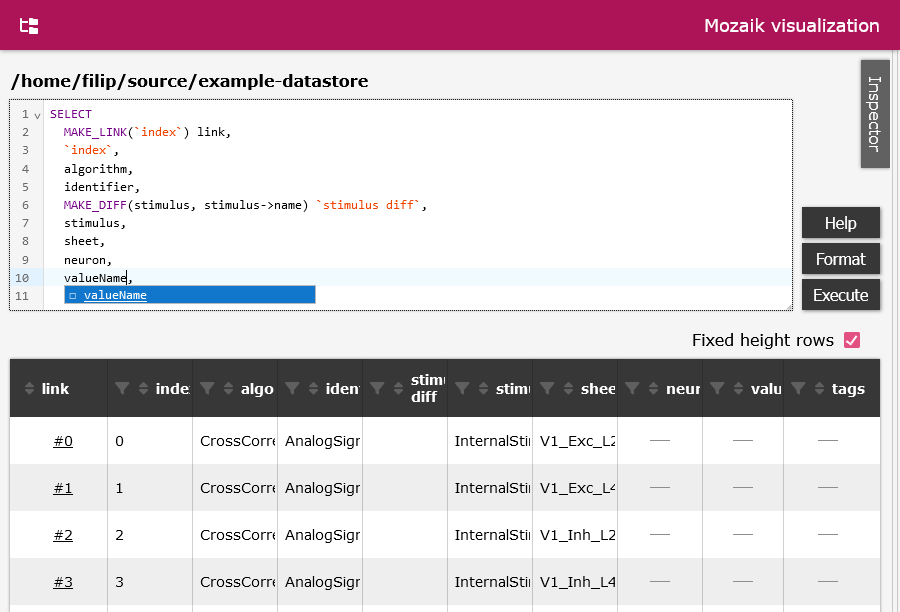
\includegraphics[width=1\linewidth]{img/screenshot_navigator.png}
	\caption{Všechny ADS jsou načteny do in-memory SQL tabulky, kterou je možné dotazovat. Po kliknutí na název sloupce je možné řádky seřadit. Vedle názvu je také vidět tlačítko pro zobrazení filtrů. V záhlaví celé stránky je nalevo vidět tlačítko pro otevření výběru datastore. To je dostupné neustále.}
	\label{fig:navigator}
\end{figure}

\begin{figure}
	\centering
	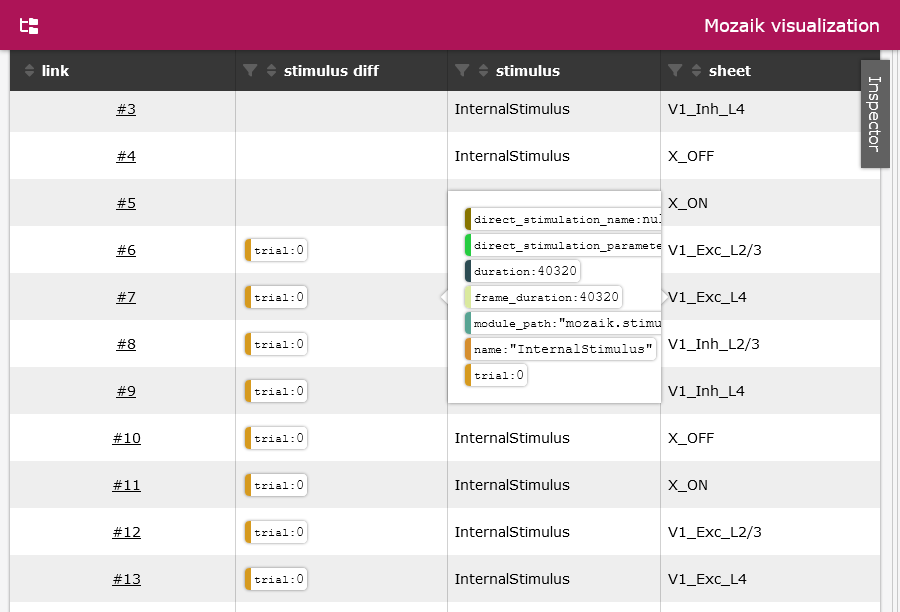
\includegraphics[width=1\linewidth]{img/screenshot_stimulus.png}
	\caption{Stimulus má většinou příliš mnoho parametrů na to, aby se do tabulky příjemně vešel. Zobrazuje se tedy jen jeho jméno a parametry jsou přístupné po najetí kurzorem.}
	\label{fig:stimulus}
\end{figure}

\begin{figure}
	\centering
	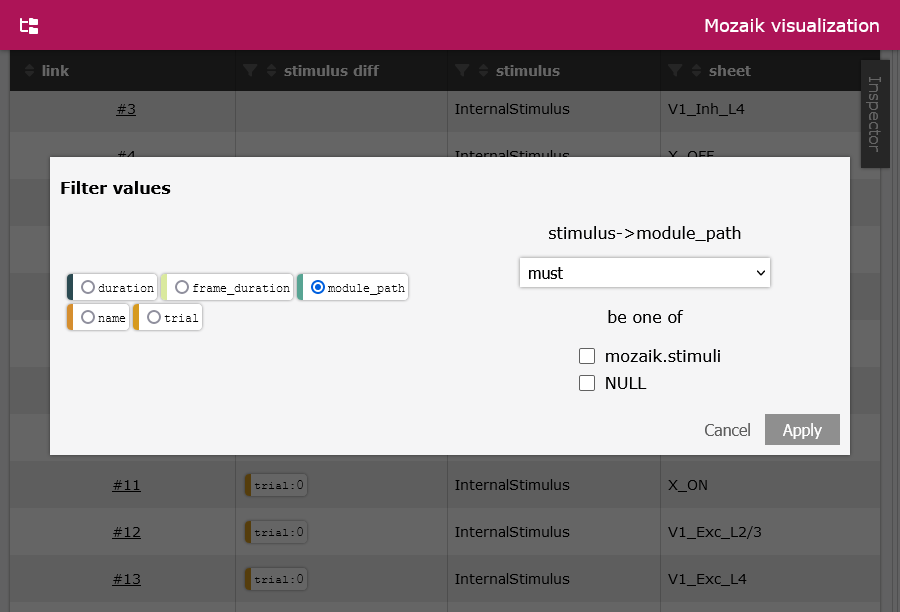
\includegraphics[width=1\linewidth]{img/screenshot_filter.png}
	\caption{Takto vypadá filtr sloupce s key-value hodnotami. Položka \lstinline|module_path| má mezi všemi stimuly jen dvě hodnoty, takže není třeba komplikovanějších podmínek.}
	\label{fig:filter}
\end{figure}

\begin{figure}
	\centering
	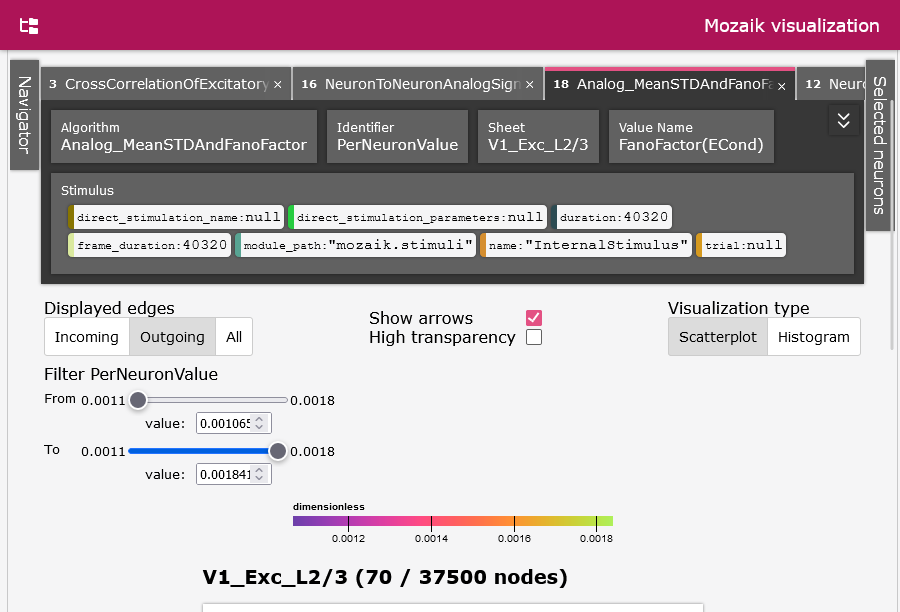
\includegraphics[width=1\linewidth]{img/screenshot_tabs.png}
	\caption{Takto vypadá inspektor jednotlivých ADS. Jména záložek jsou tvořena na základě odlišných parametrů.}
	\label{fig:tabs}
\end{figure}

\begin{figure}
	\centering
	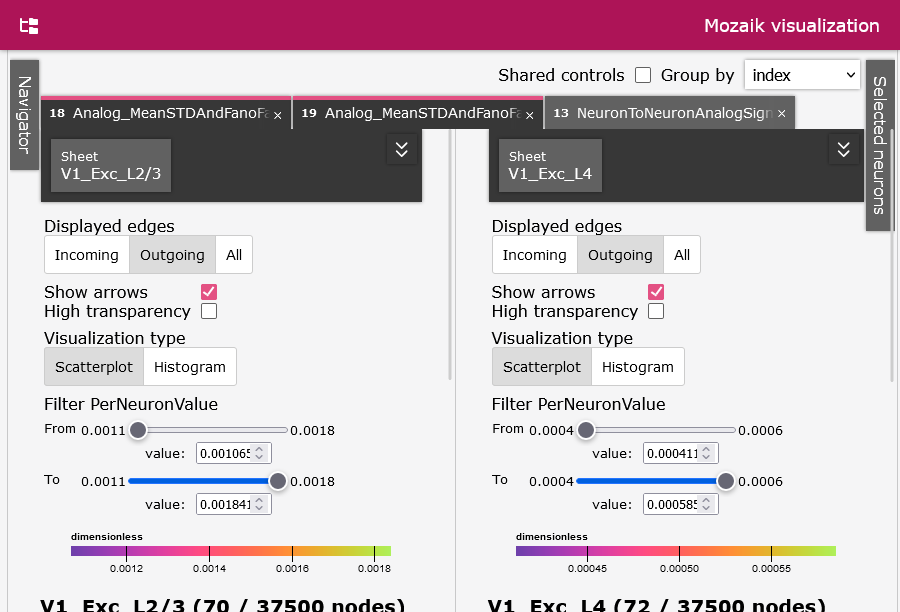
\includegraphics[width=1\linewidth]{img/screenshot_multiple_tabs.png}
	\caption{Když se vybere víc záložek naráz, základní informace o ADS ve tmavém bloku jsou redukovány na rozdílné položky.}
	\label{fig:multiple_tabs}
\end{figure}

\begin{figure}
	\centering
	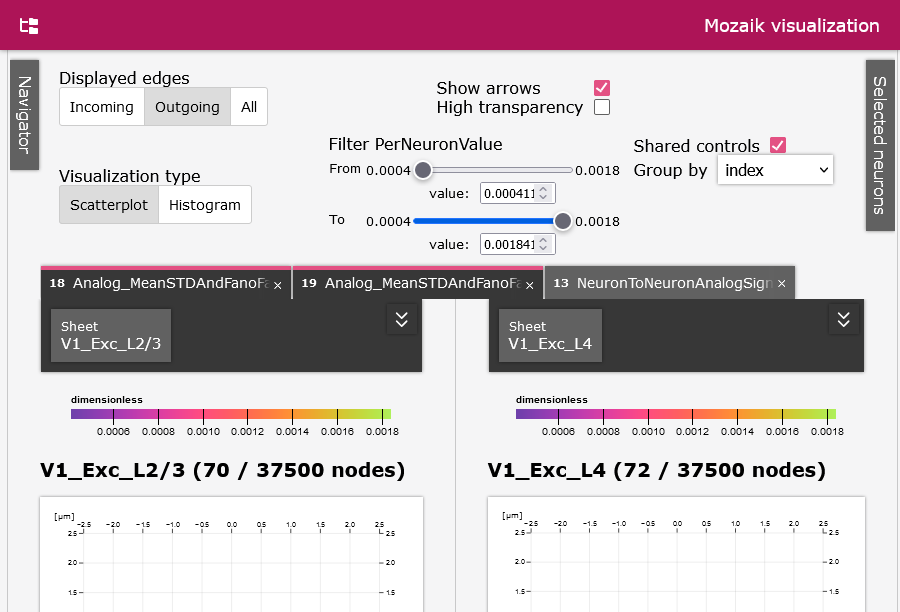
\includegraphics[width=1\linewidth]{img/screenshot_shared_controls.png}
	\caption{Když jsou sdílená nastavení záložek, přesouvají se nahoru. Je vidět, jak se oproti \ref{fig:multiple_tabs} propojilo minimum a maximum ve sliderech uprostřed.}
	\label{fig:shared_controls}
\end{figure}

\begin{figure}
	\centering
	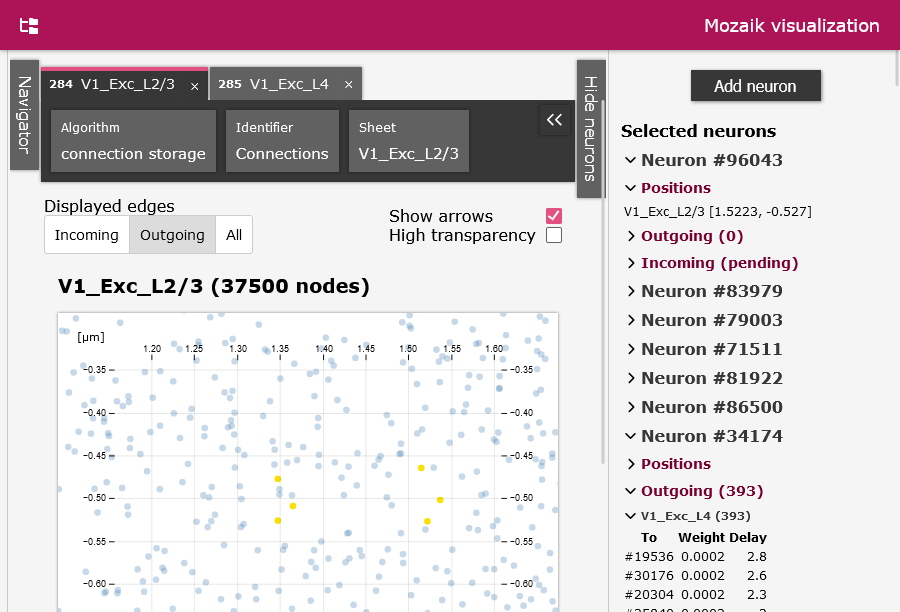
\includegraphics[width=1\linewidth]{img/screenshot_selected_neurons.png}
	\caption{Když jsou vybrané nějaké neurony, vypisují se ve speciální sekci. Vstupní spojení se spočítají až po rozbalení, protože jde o náročnou operaci. Při najetí myší na libovolný neuron se neuron zvýrazní na všech místech, kde je vidět, včetně grafu.}
	\label{fig:selected_neurons}
\end{figure}

\begin{figure}
	\centering
	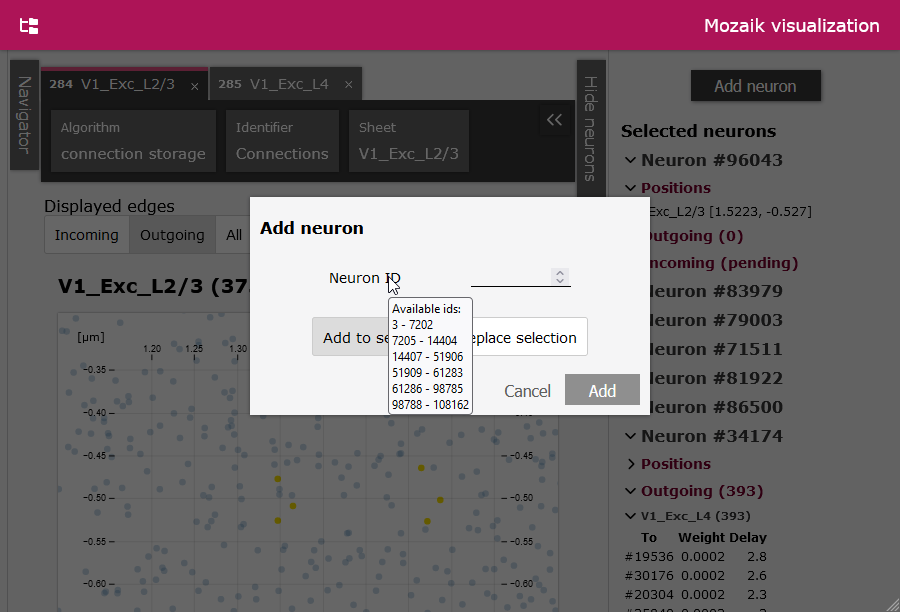
\includegraphics[width=1\linewidth]{img/screenshot_add_neuron.png}
	\caption{Neurony lze vybírat buď v grafech, nebo v tabulce spojení vypsané v sekci vybraných neuronů, nebo pomocí dialogu.}
	\label{fig:add_neuron}
\end{figure}

\begin{figure}
	\centering
	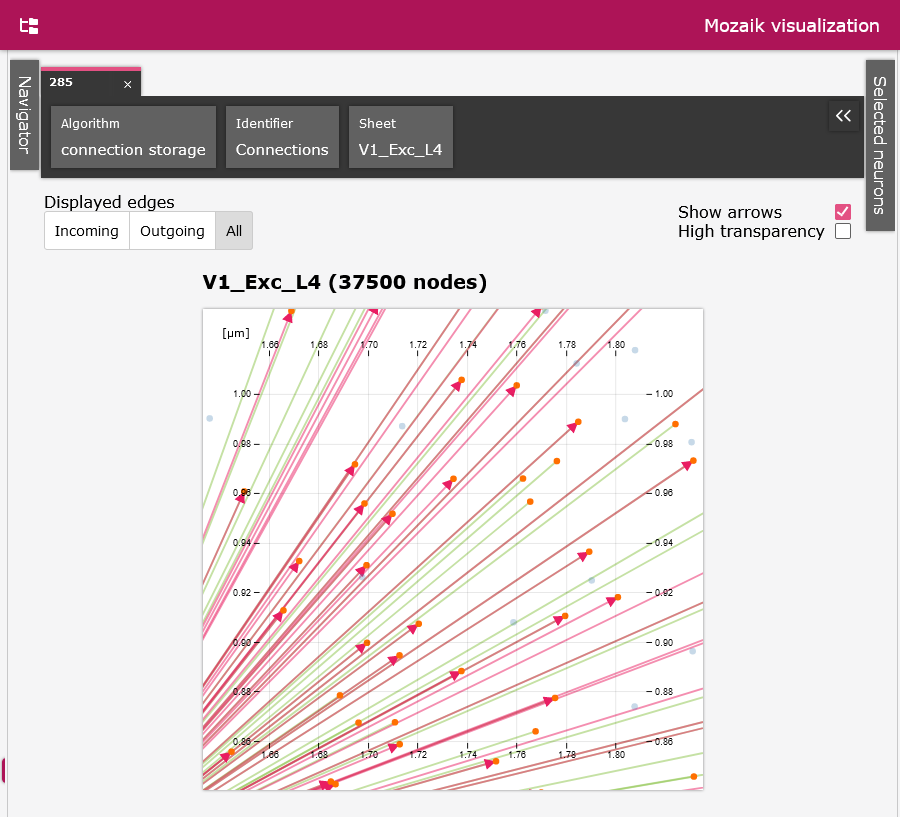
\includegraphics[width=1\linewidth]{img/screenshot_connections.png}
	\caption{Takto vypadá vizualizace spojení v neuronové vrstvě. Červené šipky vedou ven z vybraného neuronu a zelené dovnitř.}
	\label{fig:connections}
\end{figure}

\begin{figure}
	\centering
	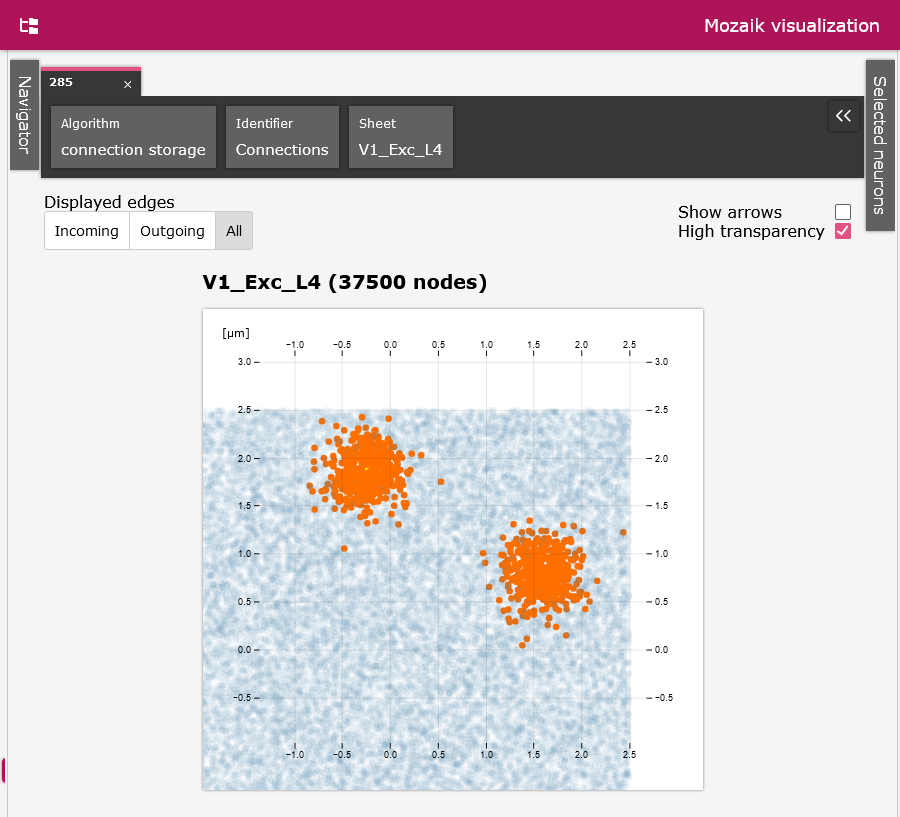
\includegraphics[width=1\linewidth]{img/screenshot_connections_dense.png}
	\caption{Když je neuronů příliš mnoho, spojení jsou špatně vidět. V nastavení vizualizace lze vypnout šipky mezi neurony a zvýšit průhlednost nevybraným.}
	\label{fig:connections_dense}
\end{figure}

\begin{figure}
	\centering
	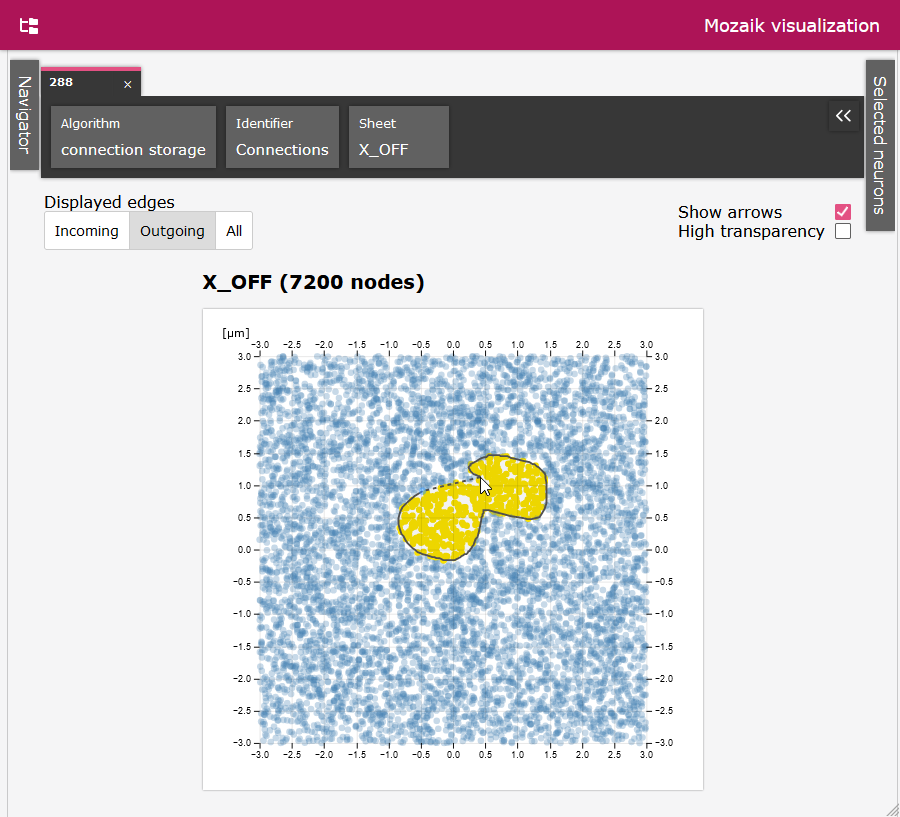
\includegraphics[width=1\linewidth]{img/screenshot_lasso.png}
	\caption{Neuron lze vybrat kliknutím. Kliknutí s klávesou shift neuron do výběru přidá nebo odebere, zachovávajíc ostatní vybrané neurony. Je také možné s klávesou shift opsat myší cestu a vybrat všechny neurony uvnitř. Klávesou escape se pak výběr zruší.}
	\label{fig:lasso}
\end{figure}

\begin{figure}
	\centering
	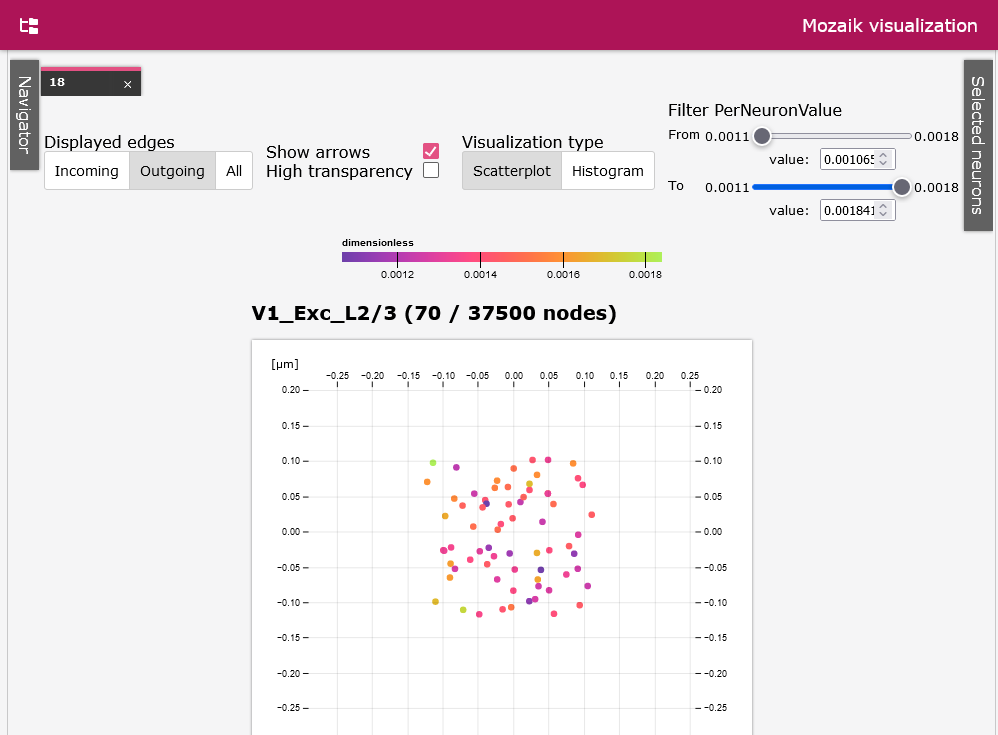
\includegraphics[width=1\linewidth]{img/screenshot_pnv.png}
	\caption{PerNeuronValue ADS je vizualizovaná jako obarvený graf neuronové vrstvy. Kdyby šlo o periodickou veličinu, barevná škála by byla cyklická. Je možné filtrovat neurony na základě jejich hodnoty.}
	\label{fig:pnv}
\end{figure}

\begin{figure}
	\centering
	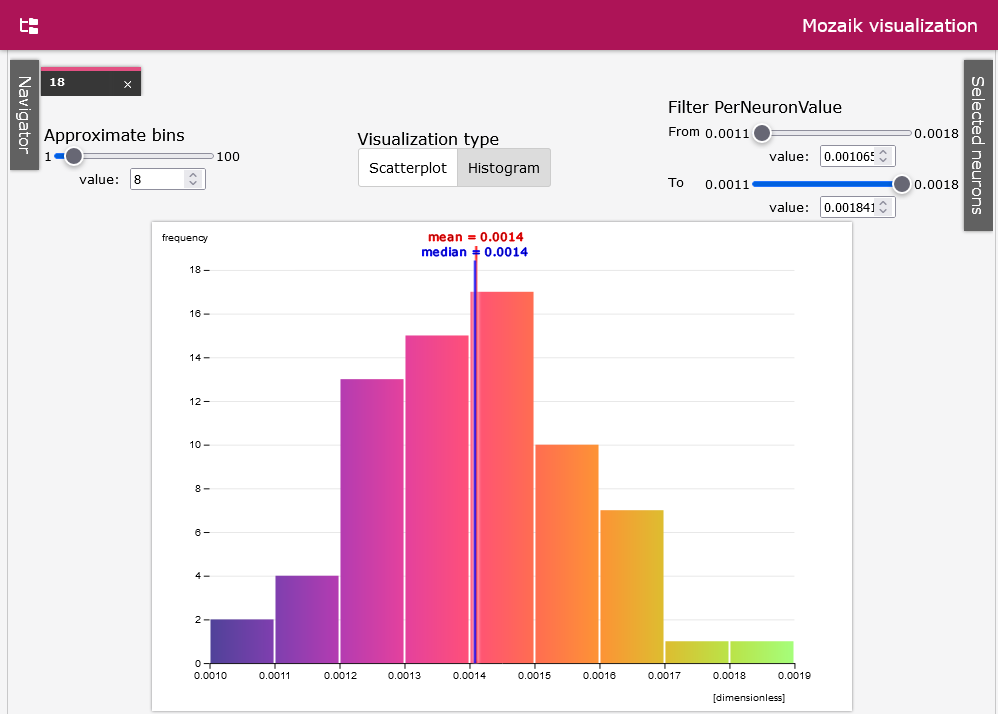
\includegraphics[width=1\linewidth]{img/screenshot_pnv_histogram.png}
	\caption{Alternativní zobrazení PerNeuronValue je v podobě histogramu. Je možné do určité míry ovlivnit počet přihrádek pomocí slideru nahoře vlevo. Histogram ukazuje také medián a aritmetický průměr hodnot.}
	\label{fig:pnv_histogram}
\end{figure}

\begin{figure}
	\centering
	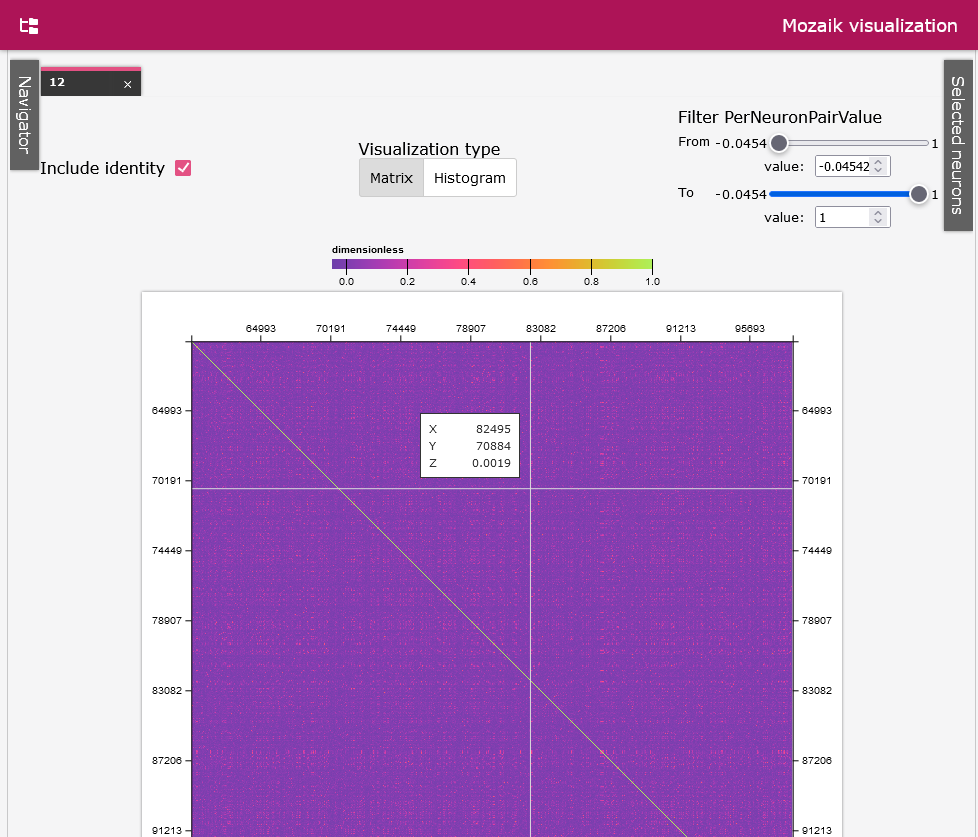
\includegraphics[width=1\linewidth]{img/screenshot_pnpv.png}
	\caption{PerNeuronPairValue je vizualizovaná jako matice. Je možné v ní podobně jako v PerNeuronValue filtrovat hodnoty, stejně tak lze nakreslit histogram. Ten je stejný jako v \ref{fig:pnv_histogram}.}
	\label{fig:pnpv}
\end{figure}

\begin{figure}
	\centering
	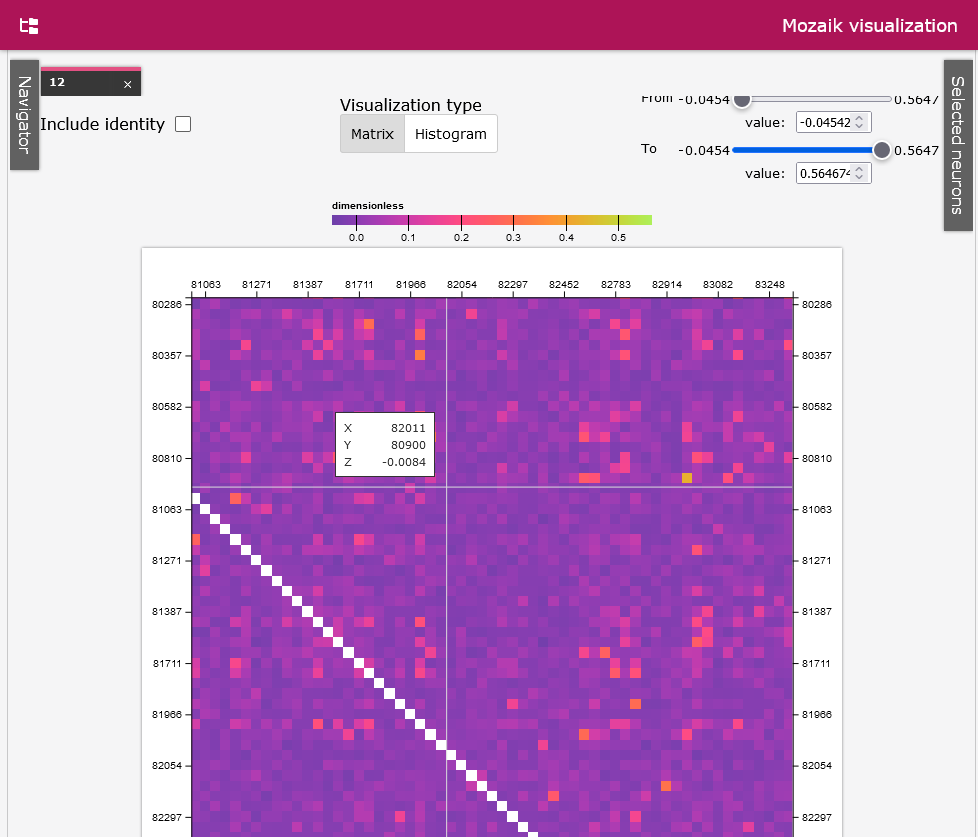
\includegraphics[width=1\linewidth]{img/screenshot_pnpv_noident.png}
	\caption{Jak bylo vidět na obrázku \ref{fig:pnpv}, občas může být na hlavní úhlopříčce hodnota, která výrazně vybočuje z ostatních. Tuto hodnotu je možné vyfiltrovat a zlepšit barevné rozložení.}
	\label{fig:pnpv_noident}
\end{figure}

\begin{figure}
	\centering
	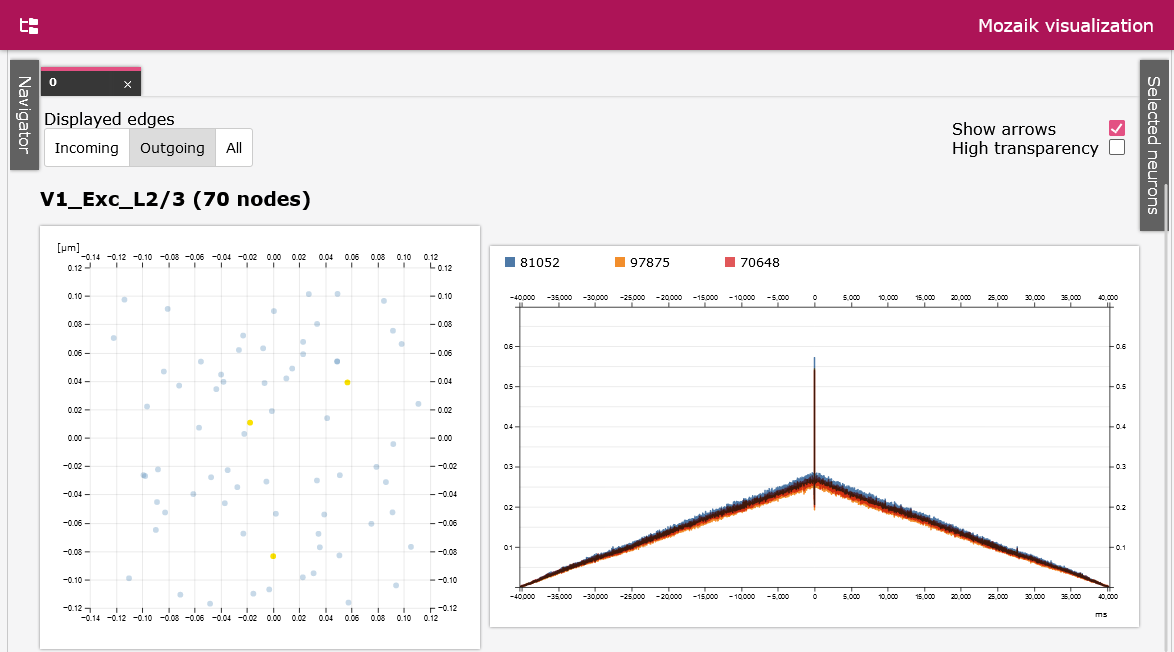
\includegraphics[width=1\linewidth]{img/screenshot_asl.png}
	\caption{AnalogSignalList je zobrazená jako graf neuronů a graf seznamů pro vybrané z nich.}
	\label{fig:asl}
\end{figure}

\begin{figure}
	\centering
	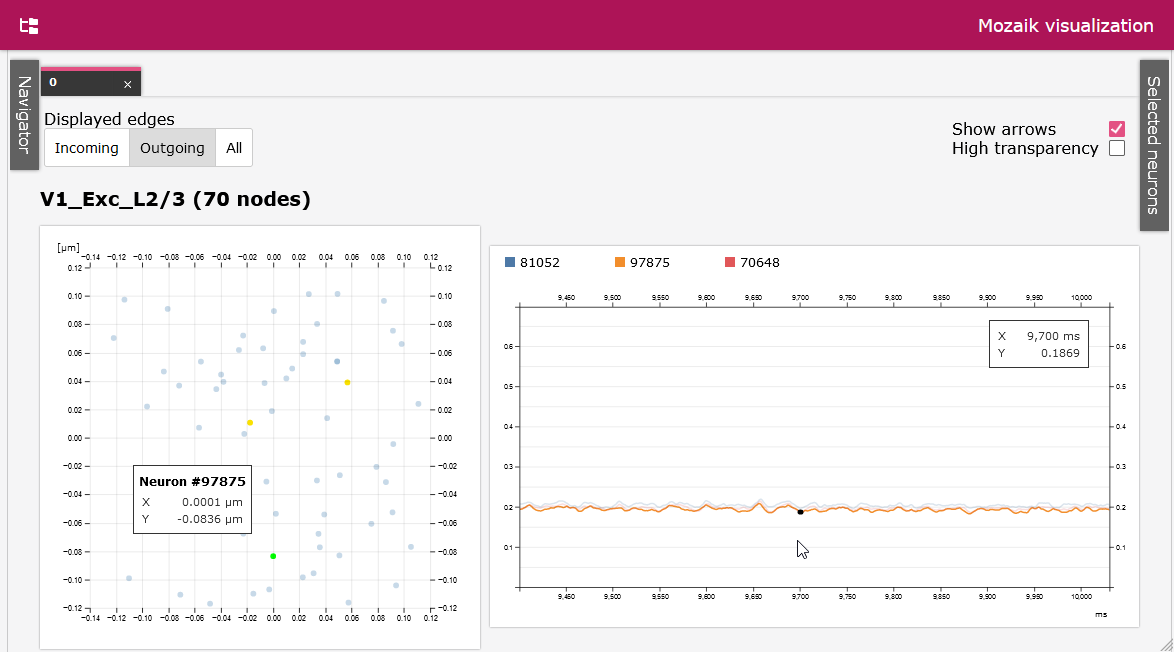
\includegraphics[width=1\linewidth]{img/screenshot_asl_zoom.png}
	\caption{Čárový graf lze zvětšovat podle osy X. Při pohybu myší se zvýrazní nejbližší bod grafu, jeho lomená čára a dotyčný neuron.}
	\label{fig:asl_zoom}
\end{figure}